% Digital Logic Report Template
% Created: 2020-01-10, John Miller

%==========================================================
%=========== Document Setup  ==============================

% Formatting defined by class file
\documentclass[11pt]{article}

% ---- Document formatting ----
\usepackage[margin=1in]{geometry}	% Narrower margins
\usepackage{booktabs}				% Nice formatting of tables
\usepackage{graphicx}				% Ability to include graphics

%\setlength\parindent{0pt}	% Do not indent first line of paragraphs 
\usepackage[parfill]{parskip}		% Line space b/w paragraphs
%	parfill option prevents last line of pgrph from being fully justified

% Parskip package adds too much space around titles, fix with this
\RequirePackage{titlesec}
\titlespacing\section{0pt}{8pt plus 4pt minus 2pt}{3pt plus 2pt minus 2pt}
\titlespacing\subsection{0pt}{4pt plus 4pt minus 2pt}{-2pt plus 2pt minus 2pt}
\titlespacing\subsubsection{0pt}{2pt plus 4pt minus 2pt}{-6pt plus 2pt minus 2pt}

% ---- Hyperlinks ----
\usepackage[colorlinks=true,urlcolor=blue]{hyperref}	% For URL's. Automatically links internal references.

% ---- Code listings ----
\usepackage{listings} 					% Nice code layout and inclusion
\usepackage[usenames,dvipsnames]{xcolor}	% Colors (needs to be defined before using colors)

% Define custom colors for listings
\definecolor{listinggray}{gray}{0.98}		% Listings background color
\definecolor{rulegray}{gray}{0.7}			% Listings rule/frame color

% Style for Verilog
\lstdefinestyle{Verilog}{
	language=Verilog,					% Verilog
	backgroundcolor=\color{listinggray},	% light gray background
	rulecolor=\color{blue}, 			% blue frame lines
	frame=tb,							% lines above & below
	linewidth=\columnwidth, 			% set line width
	basicstyle=\small\ttfamily,	% basic font style that is used for the code	
	breaklines=true, 					% allow breaking across columns/pages
	tabsize=3,							% set tab size
	commentstyle=\color{gray},	% comments in italic 
	stringstyle=\upshape,				% strings are printed in normal font
	showspaces=false,					% don't underscore spaces
}

% How to use: \Verilog[listing_options]{file}
\newcommand{\Verilog}[2][]{%
	\lstinputlisting[style=Verilog,#1]{#2}
}




%======================================================
%=========== Body  ====================================
\begin{document}

\title{ELC 4396 02 \\ Class Report 2}
\author{Jordan Cook}

\maketitle


\section*{Introduction and Problem Statement} 

The purpose of this coding project was to create a reaction timer game. A user would press start, wait a random amount of time, and press a button as soon as possible when the reaction LED lit up. This utilized several modules that needed to be created for this specific project as well as some older ones. 
\\\\ Link to my GitHub Folder: \url{https://github.com/jordanstarr/System-on-Chip/tree/master/Class_Report2}
\\ Link to the Video Clip: \url{https://github.com/jordanstarr/System-on-Chip/blob/master/Class_Report2/Video%20of%20the%20Board.mp4}

\section*{Method and Approach}

This project utilized several modules, which were created specifically for this project. 
\\\\
The first module created was essentially the timer needed to be displayed (as well as wait the random amount of time). This was done by using a counter to count the picoseconds (which was the clock cycle) and then when it reached a certain value, to increment the millisecond value. The number of milliseconds was the main output of this module. 

\begin{lstlisting}[style=Verilog,caption=Timer Module Code,label=code:ex ]
parameter bin_millisecond = 24'b00011000011010100000;

always_ff @ (posedge clk, posedge rst) begin 
	if (rst) begin
		counter <= 0; 
		ms_timer <= 0; 
	end 
	else begin
		counter <= count_next; 
		ms_timer <= ms_next;
	end   
end

always_comb begin 
	if (counter == bin_millisecond) begin 
		ms_next = ms_timer + 1; 
		count_next = 0;
	end
	else begin  
		count_next = counter + 1; 
		ms_next = ms_timer;
	end
end
\end{lstlisting}
 
Three other very important modules that were written for this lab (with code included in the Github repo, not in this report) were the Binary to Decimal Converter, the Digit to 7-segment Converter, and the 7-segment Driver. The first module (created in Digital Logic) was a way to change a binary value into a decimal through bit shifting and assignments. It is necessary to have this module since the binary values need to be displayed in decimal on the LED board.\\\\ The Digit to 7-segment Converter was created in the previous report, but updated specifically for this lab. There are three extra cases added for the board to display "H", "I" and just be blank. It was edited to drive all four of the sseg values for the anodes. \\\\ The 7-segment Driver was also created in the previous. It simply switched between the 4 anodes at a quick rate to send the proper signal to the LED's. \\\\

Since there was user input from buttons, it was important to include a debouncer so that there would be a simple single without any bounce. A debouncer module was included from Dr. Pong Chu, the author of the text book used in this class. All 3 of the buttons utilized in this program were sent through a debouncer. 

The biggest and most complex module in this project was the state machine. There were 6 states. The first was the initialization. That is where the board would say "HI" and wait for any user input. Next once a button was pressed, it would go into a wait-rand state where it would get a random number and do something until that set time had passed. During this time, it would show nothing. The next stage was the test stage, where the board would count up in milliseconds with a sensory LED on. If the button was pressed before one second had elapsed, it would go into the done state, displaying the time at which the button was pressed. If the button was not pressed in that time, it would simply display 1000, indicating the user had been too slow (and be in the late state) If the button was pressed even before the sensory LED turned on, an error would occur, 9999 would be displayed, and the state would be early.\\\\
\newpage
Below shows a diagram for the state machine. In order to better understand the behavior of the lab, this was created. 

\begin{figure}[h]\centering
	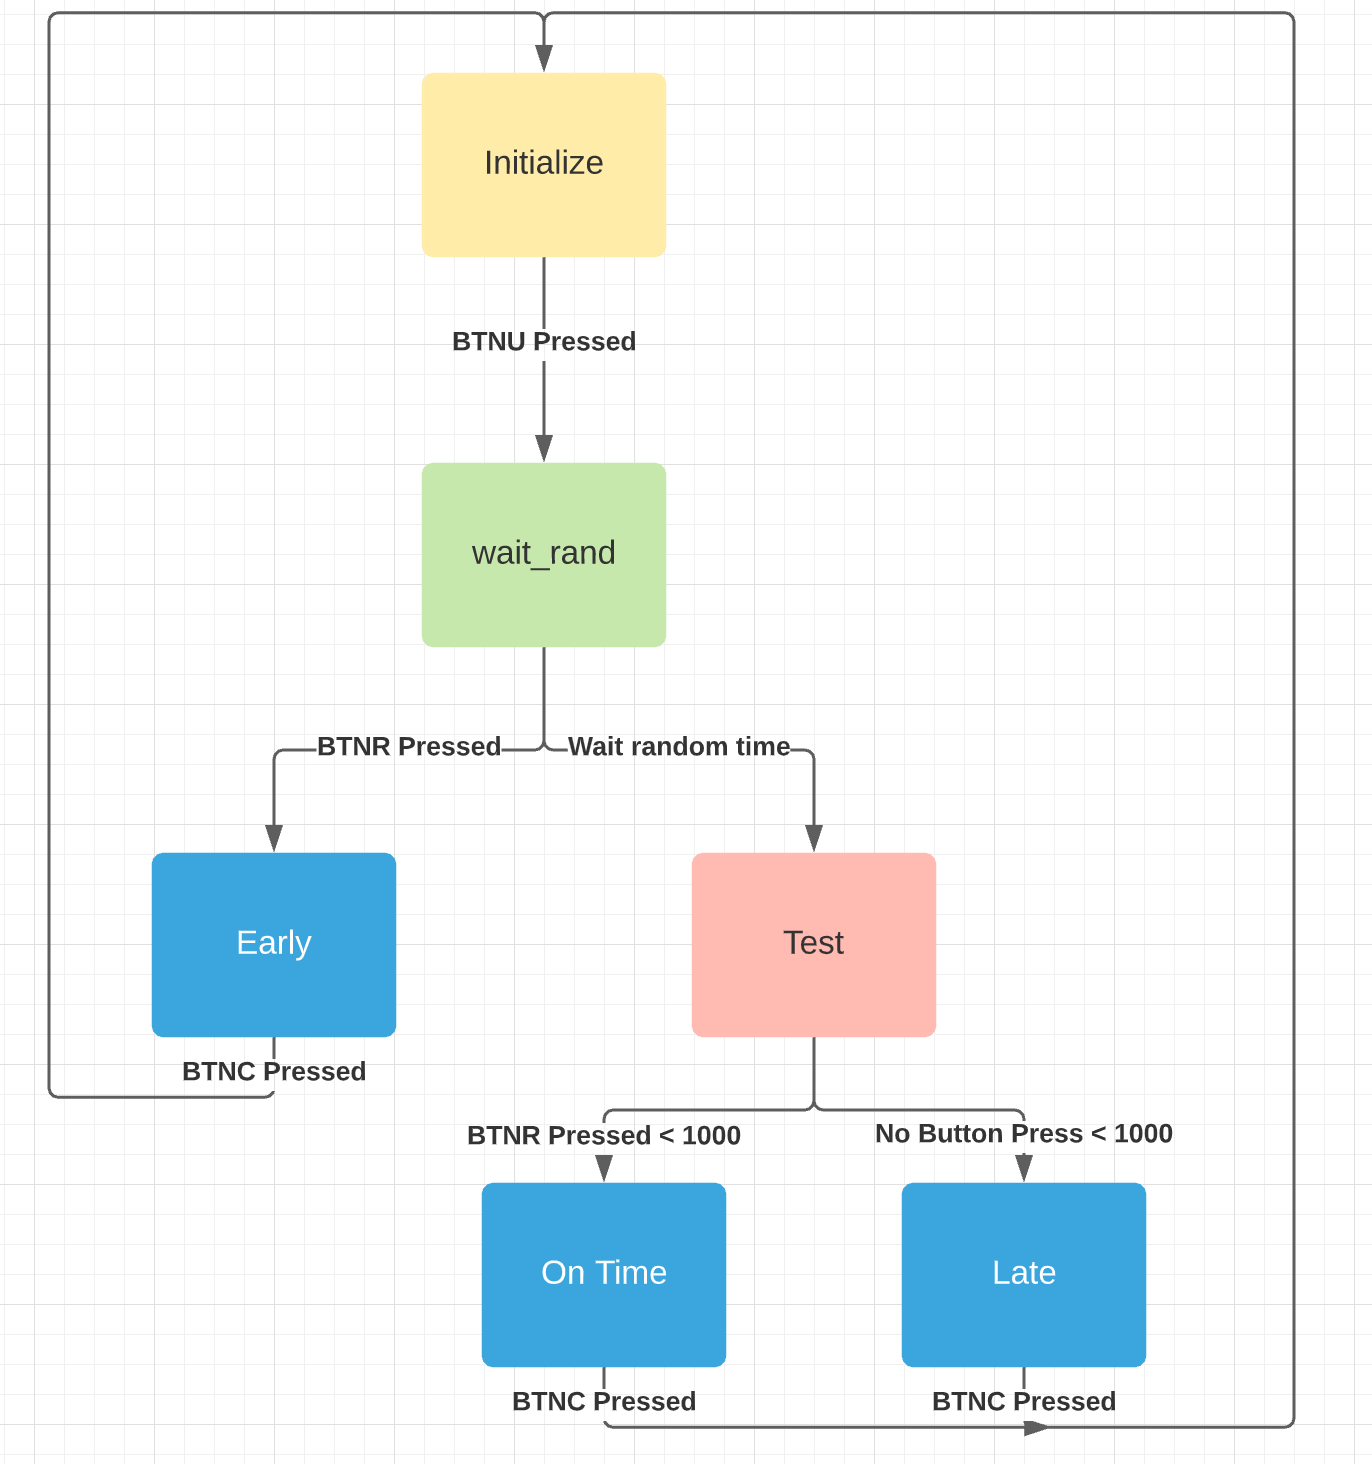
\includegraphics[width=0.85\textwidth, trim=0cm 0cm 0cm 0cm, clip]{block.PNG}
	\caption{Block Diagram for the State Machine}
	\label{}
\end{figure}
\newpage
Once the block diagram was created, it could be more easily translated over to code, as shown below. 
\begin{lstlisting}[style=Verilog,caption= State Machine Code,label=code:ex ]
	always_ff @ (posedge clk, posedge rst)
		if (rst)
			current_state <= initialize; 
		else
			current_state <= next_state; 
	
	always_comb @(posedge clk) begin 
		case(current_state) 
			initialize: begin 
				// say hi and do nothing else, waiting for input 
				decoder_in = 16'b1111111110101011; 
				LED = 0; 
				if (btnu_db) begin 
					next_state = wait_rand; 
					timer_reset = 1;
				end
			end
			wait_rand: begin 
				// incrementing ms to the random value and waiting until that time
				timer_reset = 0; 
				decoder_in = 16'b1111111111111111;
				if (ms_timer == random_num) begin 
					LED = 1; 
					next_state = test; 
				timer_reset = 1; 
				end
				else if (btnr_db) begin 
					next_state = early; 
				end
			end 
			test: begin 
				// turn LED on and count up in ms on screen
				timer_reset = 0; 
				decoder_in = bin_to_dec;
				if (ms_timer == 1000) begin 
					next_state = late; 
				end
				else if (btnr_db) begin 
					next_state = ontime; 
					stop_time = bin_to_dec; 
				end
			end
			ontime: begin 
				// display the time at which the button was pressed
				decoder_in = stop_time; 
				LED = 0; 
				if (btnc_db) begin 
					next_state = initialize; 
				end
			end 
			late: begin 
				// display 1000 and stop time
				decoder_in = 16'b0001000000000000;
				LED = 0; 
				if (btnc_db) begin 
					next_state = initialize; 
				end
			end 
			early: begin 
				// display 9999 because the button was pressed before wait was over
				decoder_in = 16'b1001100110011001; 
				LED = 0;
				if (btnc_db) begin 
					next_state = initialize; 
				end
			end
		endcase    
	end
\end{lstlisting}

There was a module created in class to generate the random number. It seemed to generate the same random number each time. This was possibly because of the algorithm used. In the future, some sort of static variable may need to be created so that it can store the random variable each time. \\

The last thing left to do was create a top level module that connected all the aforementioned modules. It created instantiatons and properly set the right logics to one another. 

\begin{lstlisting}[style=Verilog,caption= Top Module Code,label=code:ex ]
`timescale 1ns / 1ps

module top(
	input logic clk, 
	input logic reset_n,
	input logic btnc, 
	input logic btnr, 
	input logic btnu, 
	
	output logic [7:0] an, 
	output logic [7:0] sseg,
	output logic LED
	);
	
	logic [7:0] ss0; 
	logic [7:0] ss1; 
	logic [7:0] ss2; 
	logic [7:0] ss3; 
	
	logic [15:0] decoder_disp; 
	
	state_machine SM (
		.clk(clk), 
		.rst(!reset_n), 
		.btnc(btnc), 
		.btnu(btnu), 
		.btnr(btnr), 
		.decoder_in(decoder_disp), 
		.LED(LED)
		); 
	
	dig_to_sseg myDecode (
		.digit(decoder_disp), 
		.ss0(ss0), 
		.ss1(ss1), 
		.ss2(ss2), 
		.ss3(ss3)
		); 
	
	ssegDriver myDriver (
		.clk(clk), 
		.rst(rst), 
		.ss0(ss0), 
		.ss1(ss1), 
		.ss2(ss2), 
		.ss3(ss3),
		.sseg(sseg), 
		.an(an)
		);
endmodule
\end{lstlisting}

\section*{Testing}
For testing in this lab, it was useful to make sure each state was working separately before combining them all together. For example, first the board was checked if it would say "HI". Then it was tested to see if the timer would work and display. Next, buttons and debouncers were checked, plus confirming whether or not states were changed. Hard-coding was very useful in these stages until everything could be joined. Once all of these components would work separately, it was simple to integrate everything together into the state machine module. 

\section*{Results}
The results of this lab were exactly as expected: a reaction timer. It displays the time at which the button is pressed after the LED turns on, often times between 150 ms and 300 ms. A video of it functioning is included on GitHub. 

\section*{Conclusion}
This lab demonstrated many different components. The over-arching goal was to create a simple state machine. States were changed based on timing and a user pressing down certain buttons. A timer was created from the clock cycles and displayed on the LED screen when prompted. One of the most difficult parts of this lab was determining what modules were needed and how to integrate everything together. System Verilog is very different from coding in languages like C and requires a completely different approach. All in all, much was learned from generating this code and experience like this will be beneficial in the future. 

\end{document}